\documentclass[a4paper,10pt]{report}

\usepackage[utf8]{inputenc}
\usepackage{array, xcolor, booktabs}
\usepackage[hidelinks]{hyperref}
\usepackage{tikz, listings, longtable}
\usepackage{enumitem}
\usepackage{titlesec}
\usepackage{changepage}

%
% this makes list spacing much better.
%
\newenvironment{my_itemize}{
\begin{itemize}
  \setlength{\itemsep}{1pt}
  \setlength{\parskip}{0pt}
  \setlength{\parsep}{0pt}}{
\end{itemize}}

\newcommand{\footnoteremember}[2]{
\footnote{#2}
\newcounter{#1}
\setcounter{#1}{\value{footnote}}
}
\newcommand{\footnoterecall}[1]{
\footnotemark[\value{#1}]
}

\newcommand\VRule[1][\arrayrulewidth]{\vrule width #1}
\newcommand*{\myalign}[2]{\multicolumn{1}{#1}{#2}}
\newcommand\Colorhref[3][blue]{\href{#2}{\small\color{#1}#3}}

\makeatletter
\def\@makechapterhead#1{%
  \vspace*{10\p@}%
  {\parindent \z@ \raggedright \normalfont
    %\ifnum \c@secnumdepth >\m@ne
    %    \huge\bfseries \@chapapp\space \thechapter
    %    \par\nobreak
    %    \vskip 20\p@
    %\fi
    \interlinepenalty\@M
    \Huge \bfseries #1\par\nobreak
    \vskip 15\p@
  }}
  \makeatother

\def\codefont{
  \fontsize{9pt}{11pt}\selectfont}
\definecolor{codebgcolor}{HTML}{EDEDED}
\newenvironment{code}
{\begin{center}
    \begin{tikzpicture}
      \node [fill=codebgcolor,rounded corners=5pt]
      \bgroup
      \bgroup\codefont
      \begin{tabular}{l}}
      {\end{tabular}
      \egroup
      \egroup;
    \end{tikzpicture}
 \end{center}}
 
\begin{document}

\renewcommand{\thesection}{1.\arabic{section}}

\begin{center}
\begin{Large}
\textbf{CS6370 Programming Assignment - IV}
\end{Large}
\vspace{5 mm}

\emph{Sabarinath N P (CS10B020)}
\end{center}
\vspace{5 mm}
\section*{Introduction}
The objective of this assignment is to perform LDA on the given document collection and use it to cluster the documents. Gibbs
sampling method is used as the subroutine to perform LDA. The purity of this topic model is then compared against the base model.
\section*{Dataset Description}
\begin{my_itemize}
 \item The dataset contains 2761 documents each belonging one of 5 topics
 \item Size of vocabulary is 46885
\end{my_itemize}
\section*{Theory}

In each round the topic for each word is chosen using Gibbs sampling assuming topic is assigned to all other words in a document.
The probability distribution is given by
\[ P(z = k | .) = (n_{d,k} + \alpha_k) * \frac{n_{k,w} + \beta_w}{n_k+\beta*|V|} \]
where, \\
$n_{d,k}$ is number of words are assigned with topic k in document d\\
$n_{k,w}$ is number of times word w is assgined topic k\\
$n_k$ is the total number of words assgined with topic k\\
$|V|$ is the size of vocabulary
\\\\
The parameters are taken according to the given LDA reference. $\alpha = \frac{50}{|K|}$ and $\beta = 0.01$
In the second part of the assignment the goodness of clustering is measure in terms of purity which is given as follows,
\[ purity(\Omega, \mathcal{C}) = \frac{1}{N}\sum_k max_j |\omega_k \cap c_j|\]
\section*{Results}

When number of topics is fixed to 5 and the number of clusters in K-Means is varied from 2 to 49, the cluster purity
gradually increases after an inital burst, from 41\% to 76\% (when gibbs smapling run for 1000 iterations). This is mainly 
attributed by the fact that as the nuber of clusters increases the cluster size decreases and hence the number of documents assgined
with wrong topic decreases faster than number of correctly assigned documents.
The below table displays the first 10 different number of clusters
\begin{center}
\begin{tabular}{!{\VRule[2pt]}c!{\VRule[2pt]}c!{\VRule[2pt]}c!}
\specialrule{2pt}{0pt}{0pt}
\myalign{!{\VRule[2pt]}c!{\VRule[2pt]}}{\textbf{Number of Clusters}} & 
\myalign{c!{\VRule[2pt]}}{\textbf{Purity}} 
\\\specialrule{2pt}{0pt}{0pt}
2 & 0.419\\\hline
3 & 0.626\\\hline
4 & 0.692\\\hline
5 & 0.725\\\hline
6 & 0.726\\\hline
7 & 0.723\\\hline
8 & 0.729\\\hline
9 & 0.731\\\hline
10 & 0.737\\\hline
11 & 0.739
\\\specialrule{2pt}{0pt}{0pt}
\end{tabular}
\end{center}
The corresponding graph,
\begin{center}
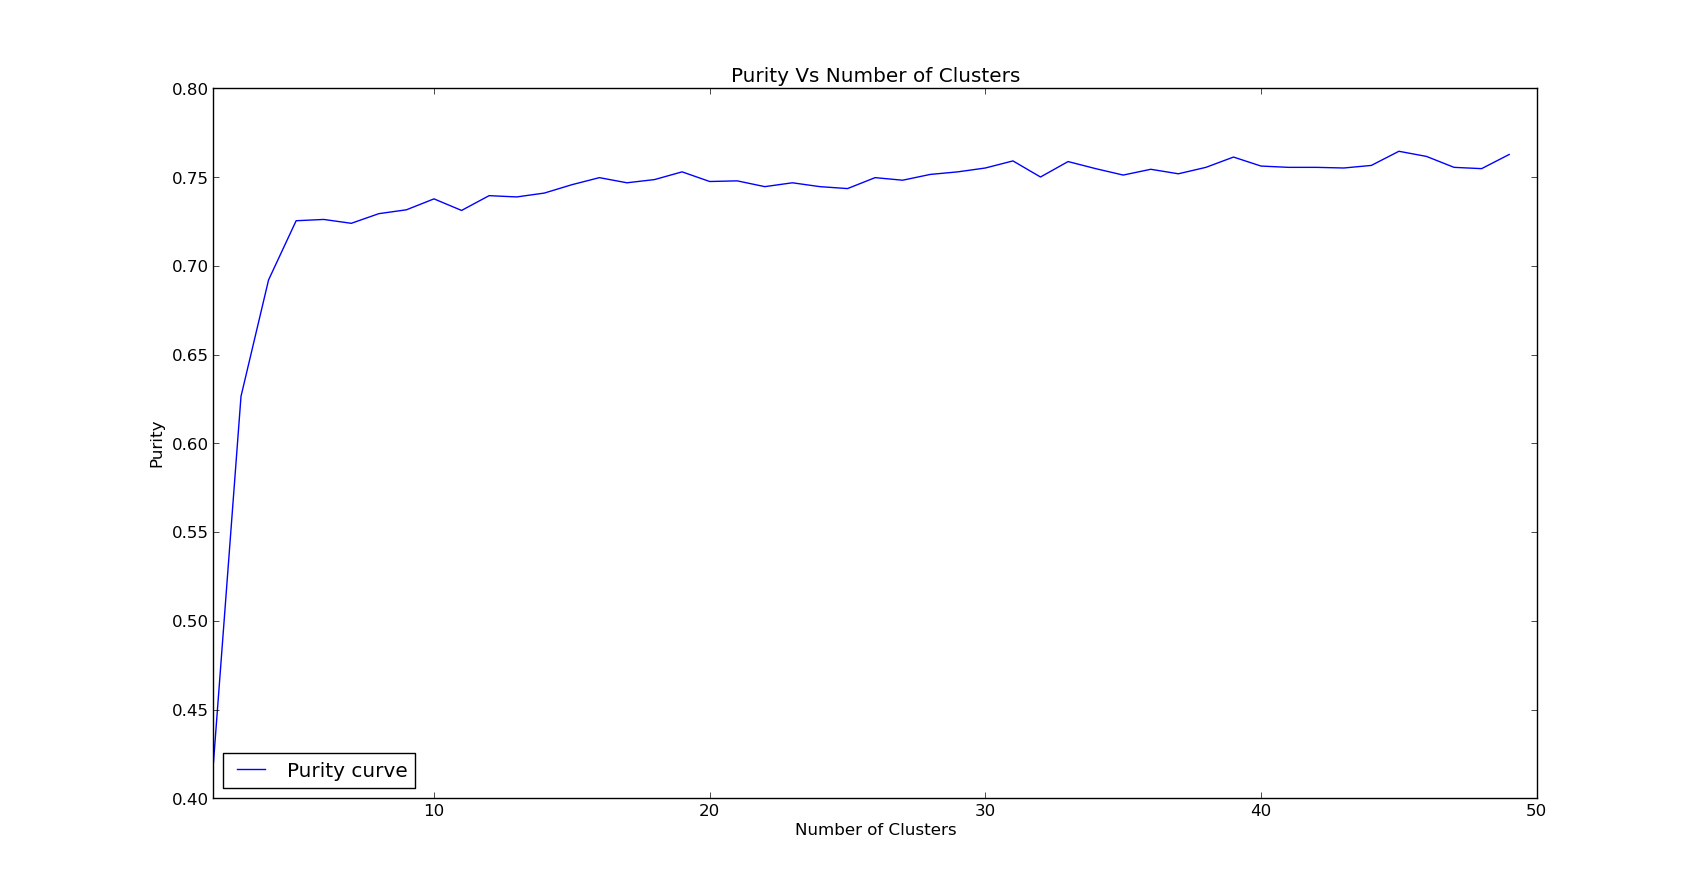
\includegraphics[height=80mm, width=120mm]{figure_1.png}
\end{center}
When number of clusters is fixed to 5 and the number of topics is varied from 2 to 10, the cluster purity increases to 79\% from 49\%
though there are osillations in the purity value. The below table shows the recorded purity values.
\begin{center}
\begin{tabular}{!{\VRule[2pt]}c!{\VRule[2pt]}c!{\VRule[2pt]}c!}
\specialrule{2pt}{0pt}{0pt}
\myalign{!{\VRule[2pt]}c!{\VRule[2pt]}}{\textbf{Number of Topics}} & 
\myalign{c!{\VRule[2pt]}}{\textbf{Purity}} 
\\\specialrule{2pt}{0pt}{0pt}
2 & 0.492\\\hline
3 & 0.617\\\hline
4 & 0.591\\\hline
5 & 0.618\\\hline
6 & 0.673\\\hline
7 & 0.705\\\hline
8 & 0.687\\\hline
9 & 0.751\\\hline
10 & 0.794
\\\specialrule{2pt}{0pt}{0pt}
\end{tabular}
\end{center}
The corresponding graph,
\begin{center}
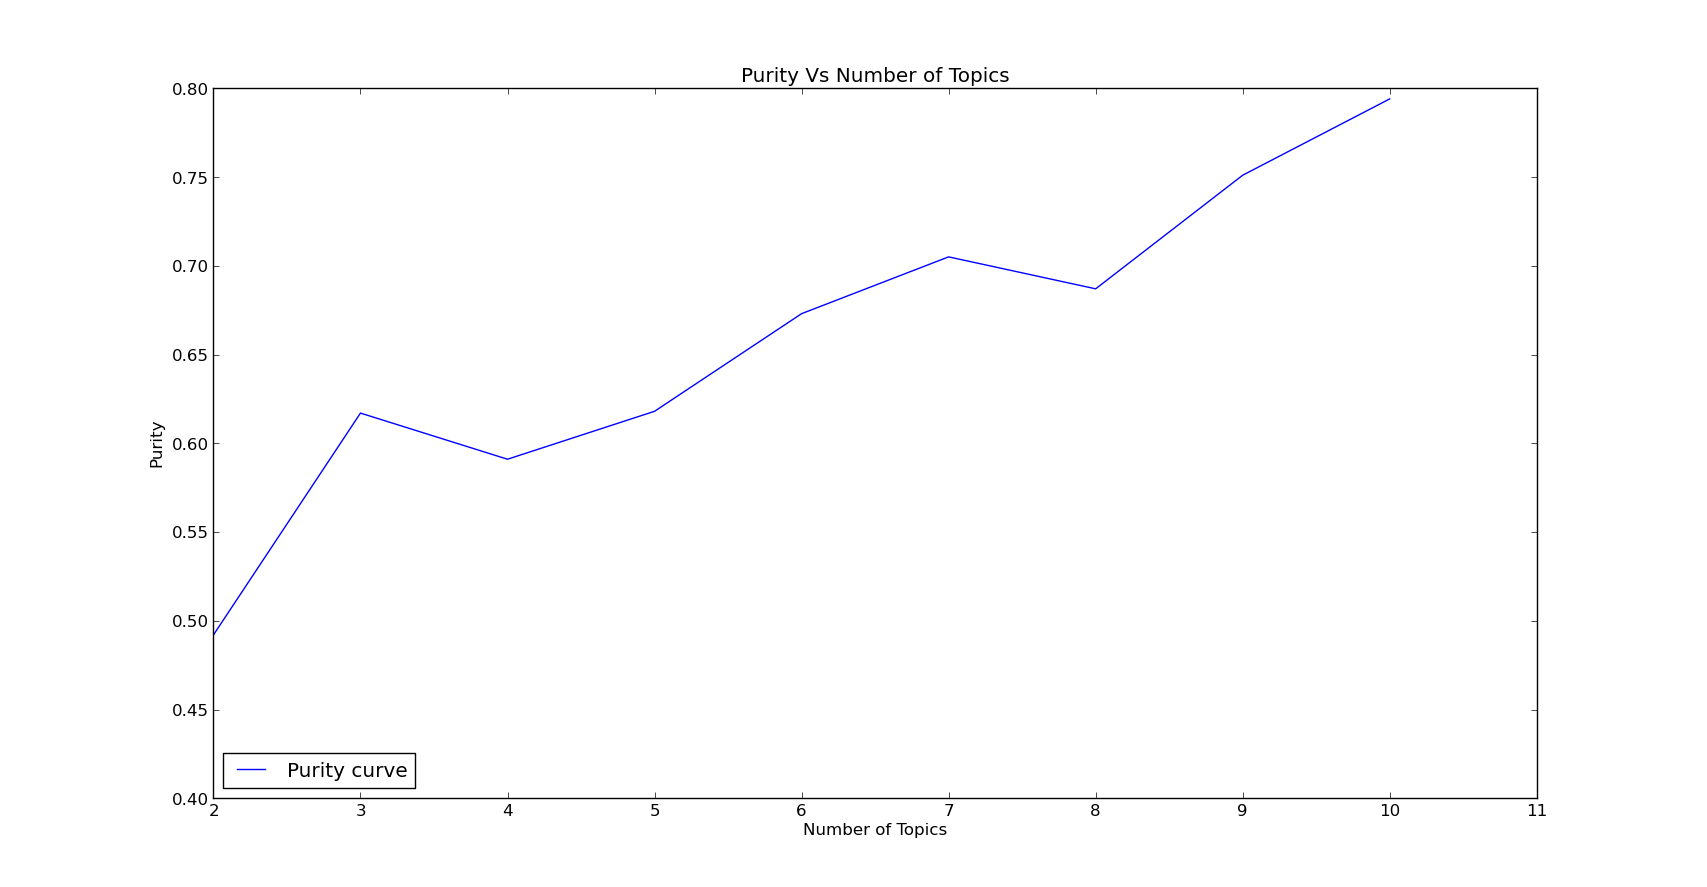
\includegraphics[height=80mm, width=120mm]{figure_2.png}
\end{center}
For instance,
\begin{my_itemize}
 \item Cluster purity when number of topics is 5, number of clusters is 5 -- 72\%
 \item Cluster purity when number of topics is 4, number of clusters is 5 -- 59.1\%
\end{my_itemize}
The top 5 words belonging to each topic. Here topic need not necessarily mean a topic with name. We just consider each topic as a
distinct number. And we are just interested in finding the words that belong to same topic as finding the actual topic of 
a given word is a different problem which is out of scope for this assignment. Below table contains the first 5 words of each topic.
\begin{center}
\begin{tabular}{!{\VRule[2pt]}c!{\VRule[2pt]}c!{\VRule[2pt]}c!{\VRule[2pt]}c!{\VRule[2pt]}c!{\VRule[2pt]}c!}
\specialrule{2pt}{0pt}{0pt}
\myalign{!{\VRule[2pt]}c!{\VRule[2pt]}}{\textbf{Topic 1}} & 
\myalign{c!{\VRule[2pt]}}{\textbf{Topic 2}} &
\myalign{c!{\VRule[2pt]}}{\textbf{Topic 3}} &
\myalign{c!{\VRule[2pt]}}{\textbf{Topic 4}} &
\myalign{c!{\VRule[2pt]}}{\textbf{Topic 5}} 
\\\specialrule{2pt}{0pt}{0pt}
nt & x & nt & organization & x\\\hline
re & nt & one & subject & window\\\hline
game & organization & people & lines & use\\\hline
writes & ones & would & university & file\\\hline
year & would & like & nntpostinghost & program
\\\specialrule{2pt}{0pt}{0pt}
\end{tabular}
\end{center}
It can be seen that the words other than the repeating stop words, belonging to same topic have the same meaning and add to the semantics of the topic.

When this topic model is compared against the base model where KMeans is run on the binary vector representation of each document,
this model performs well in terms of purity values. The base model achieved purity value of 24.3\% whereas our topic model achieved
70\% on an average.

\section*{Conclusion}
As discussed in this report, LDA serves as a powerful tool in grouping the words that belong the same topic and 
hence assign topics to the documents which any requirement of the actual semantics.
\end{document}
  